In questo capitolo si presenta il contesto in cui si è sviluppato il progetto \emph{PathS} ed alcuni concetti fondamentali collegati all'ambito di applicazione. Si citano inoltre progetti con finalità simili e approcci ritenuti interessanti punti di riferimento.

\section{Web\textsuperscript{2} e Opportunistic Sensing}
Una rete di sensori o \emph{Sensor Network} è composta di elementi autonomi e distribuiti atti al monitoraggio di determinati parametri ambientali. Ciascun nodo ha capacità autonome di calcolo, percezione e misurazione dell'ambiente circostante, comunicazione ed eventualmente di mobilità. Molte ricerche si sono focalizzate in questo ambito, in particolare con lo scopo di definire un sistema affidabile e decentralizzato per la comunicazione e il supporto a servizi in questo scenario. Raramente questo tipo di soluzioni sono andate oltre l'ambito della sperimentazione fino all'applicazione su larga scala. Il recente sviluppo tecnologico e la diffusione capillare dei dispositivi \emph{smartphone} ha radicalmente modificato la situazione, aprendo la possibilità ad importanti evoluzioni. Di fatto anche un dispositivo base ha tutte le caratteristiche necessarie, essendo dotato di un sistema GPS, moduli di connessione alla rete dati e numerosi sensori tra cui quello di prossimità, luminosità, microfono, fotocamera e accelerometri. In questo modo si possono coprire ampie zone geografiche con un buon numero di dispositivi, offrendo sia l'occasione di applicare le ricerche sviluppate nell'ambito delle \emph{sensor neteorks}, sia di esplorare scenari del tutto nuovi. Ciò che rende ancora più interessante l'applicazione di una rete pervasiva di dispositivi, non è solo la possibilità di migliorare i servizi per gli utilizzatori diretti, ma la possibilità di studiare scenari del tutto nuovi a giovamento dell'intera società.

Pensiamo a quella che è già stata una grande evoluzione del mondo di internet, ovvero il \emph{Web 2.0}. Il suo avvento è fatto coincidere con la diffusione dei social networks, alla cui base c'è l'elevato livello di interazione tra il sito Web e gli utenti stessi. In ogni caso è richiesta una interazione diretta dell'utilizzatore, il quale consapevolmente contribuisce ad aumentare la base delle informazioni. Lo sviluppo di alcune tecnologie specifiche (tra cui \emph{AJAX}) ha permesso lo scambio di dati in background fra Web browser e server consentendo l'aggiornamento dinamico della pagina senza esplicito ricaricamento da parte dell'utente. Fondamentalmente si è passati da un Web statico a uno di tipo dinamico e sociale in cui l'utente non è più solo un lettore e un consumatore passivo di contenuti, ma è il principale creatore di essi.
La diffusione capillare di questi dispositivi con sensori avanzati, apre la strada al paradigma \emph{Web\textsuperscript{2}} in cui la quantità di dati, raccolta anche senza l'esperienza utente diretta, non aumenta in modo lineare ma letteralmente esplode con andamento esponenziale. Diventa quindi di fondamentale importanza le modalità con cui si raccoglie questa mole di dati e i principi di design con cui si imposta lo sviluppo di applicazioni in questo contesto. Una buona analisi tecnica e un'architettura di rifermento per lo sviluppo di servizi \emph{Web\textsuperscript{2}} basati su reti di sensori \emph{smartphone} è fornita da Calma, Palazzi e Bujari in \cite{web2palazzi}. Nell'articolo è introdotto e sviluppato il concetto di \emph{opportunistic sensing} il quale è ritornato molto utile anche nel progetto \emph{PathS}. Gli autori espongono due criteri fondamentali secondo cui categorizzare le applicazioni in ambito \emph{Web Squared}: il primo riguarda la scala di rilevamento, il secondo è il grado di coinvolgimento degli utenti. Considerando la scala di rilevamento possiamo distinguere una applicazione in:

\begin{itemize}
\item \textbf{personale}: progettata per utenti singoli e i risultati vengono visualizzati solo all'utente stesso, senza la loro condivisione. Un esempio di queste può essere \emph{Dankam}, applicazione che aiuta nell'identificazione dei colori le persone affette da daltonismo;
\item \textbf{di gruppo}: ad esempio \emph{Nike+ o Runtastic}, applicazioni in cui un gruppo di persone con interessi affini condivide informazioni spesso sfruttando la connessione ai popolari social network;
\item \textbf{di comunità}: i dati sono raccolti da una vasta gamma di persone e i risultati condivisi pubblicamente per renderli disponibili a tutti gli utenti. Un'esempio di applicazione è Google Maps e la relativa segnalazione dei tratti trafficati.
\end{itemize}
\begin{figure}[h]
\centering
\begin{subfigure}{.33\textwidth}
  \centering
  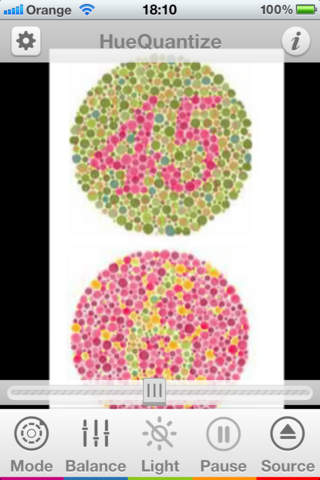
\includegraphics[height=6cm]{images/dankam2}
  \caption{\footnotesize{Dankam}}
  \label{fig:dankam}
\end{subfigure}%
\begin{subfigure}{.33\textwidth}
  \centering
  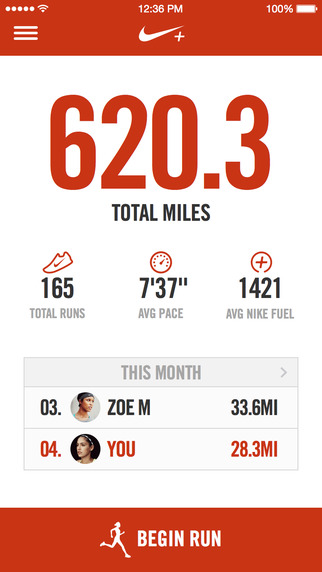
\includegraphics[height=6cm]{images/nikeplus}
  \caption{\footnotesize{Nike+}}
  \label{fig:nike+}
\end{subfigure}
\begin{subfigure}{.33\textwidth}
  \centering
  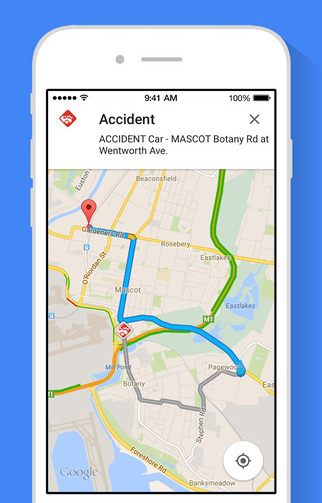
\includegraphics[height=6cm]{images/googlemaps}
  \caption{\footnotesize{Google Maps}}
  \label{fig:googlemaps}
\end{subfigure}
\end{figure}

Valutando invece il coinvolgimento con l'utente, le applicazioni di questa categoria si possono suddividere in:
\begin{itemize}
  \item \textbf{partecipative}: ovvero la raccolta dei dati avviene tramite il coinvolgimento esplicito e diretto dell'utente. Ci si affida quindi all'entusiasmo e alla relazione diretta con gli utilizzatori i quali volontariamente eseguono l'applicazione e raccolgono i dati necessari. Solitamente le informazioni che derivano da questa tipologia sono molto accurate e ben distribuite anche per la possibilità di una opportuna pianificazione. La controparte è che spesso non è facile ottenere una sufficiente base di copertura se non si dispone del bacino di utenza e delle risorse necessarie. 
  \item \textbf{opportunistiche}: in cui l'acquisizione delle informazioni avviene tramite i sensori del dispositivo in determinate situazioni di utilizzo, anche se in quel momento non è l'attività principale. La raccolta avviene quindi in \emph{background} informando, ma non richiedendo necessariamente l'attenzione, dell'utente. In qualche modo si ``distrae'' l'utilizzatore con una attività primaria dall'alto livello di gradimento e nel frattempo si approfitta della situazione per catturare le informazioni necessarie. L'aspetto negativo di questo approccio è principalmente tecnico, dato che la sovrapposizione di più attività comporta un maggiore dispendio di risorse del dispositivo (\emph{cpu}, batteria, rete ...) e al tempo stesso gli algoritmi che devono interpretare i dati provenienti dai sensori e identificare le situazioni idonee sono particolarmente complessi. Questo tipo di approccio risulta particolarmente utile per le applicazioni \emph{di comunità} che, pur raccogliendo pochi campioni, possono contare su un'ampio bacino di utenza.
\end{itemize}
Nello sviluppo del progetto \emph{PathS} ed in particolare per la progettazione della componente \emph{client} si è pensato di sfruttare entrambi questi aspetti. Tramite il coinvolgimento diretto di alcuni studenti e il coordinamento del Prof. Palazzi e dei suoi collaboratori, è stata organizzata una campagna di campionamento massivo della zona universatiria e dei dintorni. Questo ha consentito sia di raccogliere numerosi \emph{feedback} riguardo il funzionamento del sistema che di raccogliere una consistente base di informazioni per l'area di riferimento. Per integrare e ampliare questa base di partenza, si è pensato ad un approccio di tipo opportunistico presentato in dettaglio nel capitolo successivo.

Un altro aspetto fondamentale proposto nello stesso articolo è il principio di architettura software secondo cui impostare un servizio basato sul paradigma \emph{Web\textsuperscript{2}}. Concepire una applicazione mobile di questo tipo non è banale, in quanto affiancare le due attività di raccolta intensiva di dati dai sesnsori e la condivisione di essi può portare a diversi problemi. Uno degli aspetti fondamentali riguarda la gestione delle risorse (spesso limitate) del disposotivo. Un utilizzo tropppo intenso delle componenti relative ai sensori così come una trasmissione dati frequente può portare ad esaurire in breve tempo la batteria, o in alcuni casi a sovraccaricare l'unità di calcolo del del dispositivo, causando un disservizio nelle funzionalità principali (come ricevere le chiamate). 
\begin{figure}[h]
  \centering
  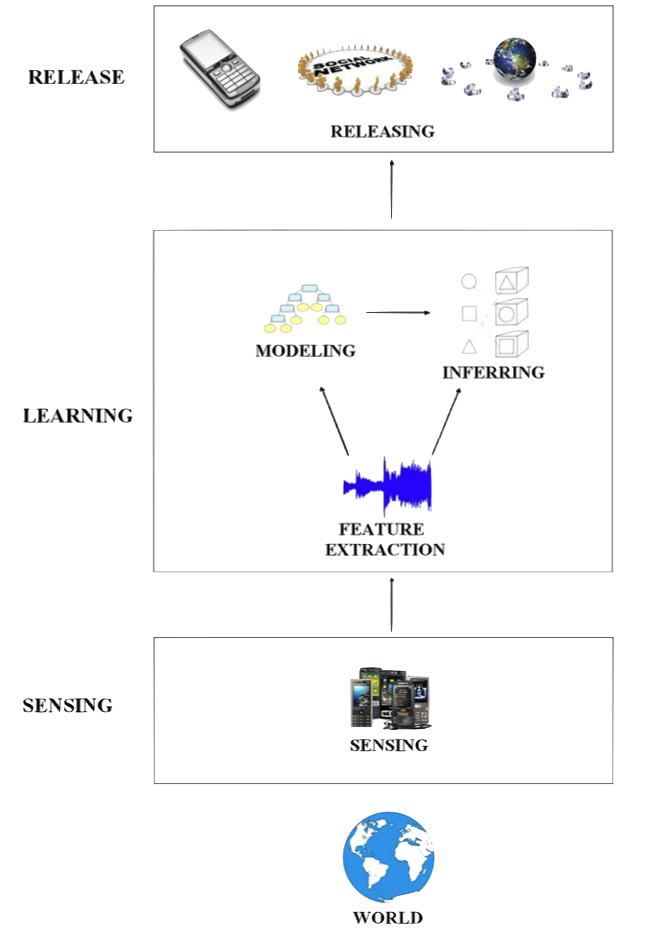
\includegraphics[height=10cm]{images/layers}
  \caption{\footnotesize{Architettura a \emph{layer} di una applicazione \emph{Web\textsuperscript{2}}}}
  \label{fig:layers}
\end{figure}
Una delle soluzioni proposte è prima di tutto individuare e separare le componenti sulla base del ruolo che devono svolgere per raggiungere il risultato atteso. Nel caso delle applicazioni \emph{Web\textsuperscript{2}} è individuato un sistema architetturale basato su tre \emph{layer} di competenza che sono:
\begin{itemize}
  \item \textbf{sensing layer}: che necessariamente risiede nel dispositivo e si occupa della raccolta dei dati grezzi dai sensori;
  \item \textbf{learning layer}: che svolge il ruolo di processare i dati raccolti e derivarne i risultati;
  \item \textbf{release layer}: che si occupa di fornire i risultati ottenuti all'utente.
\end{itemize}
Le problematiche che riguardano il primo \emph{layer} riguardano principalmente l'integrazione con gli ambienti di sviluppo (\emph{SDK}) e le modalità di accesso alle componenti del dispositivo. Spesso gli strumenti messi a disposizione degli sviluppatori non sono così a basso livello da consentire un'utilizzo ottimale. E' necessario spesso trovare dei \emph{workaround} specifici, piattaforma per piattaforma, che portino al giusto compromesso tra la frequenza di campionamento, la precisione dei dati raccolti e l'utilizzo delle risorse.
Per quanto riguarda il \emph{learning layer} si possono invece trovare le soluzioni più diverse. Non è indispensabile che questa logica applicativa risieda necessariamente nel dispositivo ma è possibile delegare l'attività ad un sistema esterno (es. server cloud) in cui la disponibilità di risorse è maggiore ed è possibile adottare algoritmi più complessi. In alcuni casi si sugggerisce anche un approccio ``misto'' in cui i dati vengono pre-processati dal dispositivo cercando di estrarre delle \emph{feature} che vengono quindi comunicate all'esterno ed elaborate.
Il \emph{release layer} si occupa di mostrare il risultato all'utente finale e, a seconda del tipo di applicazione, potrebbe avere come destinazione sia un singolo cliente così come una vasta comunità. Per questo motivo anche in questo caso le soluzioni proposte possono riguardare sistemi esterni oad esempio il collegamento a vaste reti di distribuzione tipo \emph{social-network}.

Nel progetto \emph{PathS} ritroviamo tutte queste problematiche e le soluzioni adottate seguono in molti casi i principi generali qui presentati. Ad esempio le modalità di campionamento GPS eseguite dal \emph{client} sono state tarate al fine di ottenere risultati accettabili minimizzando l'uso delle risorse. Dal punto di vista dell'architettura del sistema si è deciso di elaborare tutti i dati nel sistema \emph{server} esterno, dove i dati raccolti vengono processati e utilizzati per derivare le informazioni di sintesi. Infine agli utenti finali si comunicano i risultati sia in forma diretta (con opportuno protocollo di comunicaizone con il client) che in forma più estesa tramite l'accesso a dei servizi web.


\section{Gestione dei dati di movimento}
Un'altra tematica affrontata in quanto affine all'ambito del progetto è quella dei \emph{Mobility Data}. Alcuni esempi di \emph{mobility data} sono forniti in \cite{mdme} da Pelekis e Theodoridis e possono essere:
\begin{itemize}
  \item i dati provenienti da una conversazione telefonica cellulare (la compagnia telefonica ha informazioni aggiuntive in merito al posizionamento del dispositivo);
  \item i dati provenienti da un dispositivo GPS durante una determinata attività (la combinazione tra la posizione e il momento in cui è rilevata);
  \item i dati scambiati tra i veicoli di una \emph{vehicular ad hoc network} (\emph{VANET});
  \item i dati raccolti da un sistema di \emph{radio-frequency identification} (\emph{RFID}).
\end{itemize}
Come vediamo il concetto di \emph{mobility data} è molto vario e può essere applicato a numerosi contesti. Più in generale si considera riguardante questa tematica tutti i casi in cui si combinano assieme i dati dell'asse temporale con i dati spaziali. L'evoluzione del movimento di un oggetto nel tempo è diventato recentemente una importante tematica di ricerca. La gestione di questi dati in domini separati è ben consolidata: da una parte gli \emph{Spatial Databases} sono in grado di gestire in modo efficiente i dati posizionali e le operazioni di interrogazione su di essi, così come dall'altra parte i \emph{Temporal Databases}. Tuttavia la combinazione simultanea di questi due insiemi può aprire ad importanti prospettive di applicazione. Prendiamo ad esempio l'analisi del traffico in una rete di trasporto cittadina. E' possibile (ed è già stato realizzato in diversi studi) dotare un numero consistente di veicoli circolanti di un un dispositivo GPS. Il dispositivo registra le informazioni in merito alla posizione con una frequenza sufficientemente dettagliata (ad esempio 0.2 Hz, una campionamento ogni 5 secondi). La raccolta di queste informazioni può portare ad un \emph{set} di dati che se interpretato correttamente può fornire un supporto a richieste del tipo:
\begin{itemize}
  \item \textbf{analisi del traffico}: quanti veicoli affollano un determinato tratto in un momento specifico? Qual'è il tempo di attesa medio ad un semaforo oppure funziona correttamente l'effetto ``onda verde''?
  \item \textbf{servizi \emph{location-aware}}: qual è l'attività commerciale più vicina alla mia posizione attuale o al percorso che ho intenzione di seguire? Quali dei mia amici \emph{facebook} è in prossimità della città che sto visitando?
\end{itemize}

Quelli riportati sono solo alcuni esempi, ma più in generale lo studio di \emph{mobility data} e di \emph{database} di traiettorie può supportare lo sviluppo di \emph{Location Based Services} ed applicazioni \emph{Location-} e \emph{Mobility-Aware}. Per \emph{\textbf{Location Based Service}} si intendono tutti quei servizi che forniscono informazioni ai propri utenti sulla base della posizione geografica corrente. Se il servizio è caratterizzato da un altro grado di interazione tra gli utenti stessi e la formazione di una sorta di rete fra gli stessi, allora si può parlare di \emph{\textbf{Location-based Service Networking}}. Una tassonomia di questi servizi è proposta in tabella \ref{tablelbs} e deriva dal grado di mobilità (stazionario o mobile) degli attori coinvolti ovvero l'utente che interroga il servizio e gli oggetti interrogati a database.

\begin{table}[h!]
\centering
\begin{tabular}{ |l||l|l| } 
 \hline
 \diagbox{Database Objects}{Reference Object} & \emph{Stationary} & \emph{Mobile} \\ 
 \hline
 \hline
 \emph{Stationary} & 
  routing & 
  guide-me \\ 
 \hline
 \emph{Mobile} &
  find-me &
  get-together \\ 
 \hline
\end{tabular}
\caption{Tassonomia di applicazioni \emph{location-aware}}
\label{tablelbs}
\end{table}

Come vediamo l'ambito del progetto \emph{PathS} ha molti aspetti in comune con quelli trattati nel \emph{mobility data managment}. Tuttavia le problematiche che si intendere risolvere (almeno nelle prime fasi del progetto) riguardano la prima classe di problemi (\emph{<stationary, stationary>}) relativamente più conosciuta e trattata in letteratura. 

Modellando la rete di trasporto (\emph{transportation network}) come un grafo $G = (N, E)$ composto da nodi $N$ e archi $E$, l'operazione di \emph{routing} consiste tipicamente nel cercare un percorso ottimale che porti dalla sorgente $S$ alla destinazione $T$ dove $S, T \in N$. Tecnicamente per queste tematiche sono disponibili diversi algoritmi, principalmente basati sulla soluzione del problema di flusso \emph{Shortest Path}. Un adeguamento del calcolo dei pesi utilizzati negli archi della rete, consente di ottenere diverse modalità di navigazione ad esempio la più veloce, la più breve o, come è di recente interesse, la più ecologica.

Per questi motivi nel corso dello sviluppo del progetto \emph{PathS} ci si è allontanati da quelle che sono le problematiche e gli strumenti specifici nell'ambito del \emph{mobility data managment}, seguendo piuttosto altri spunti da cui derivare l'implementazione. Ciò non toglie che l'ambito di applicazione è molto coerente con questo tema e l'adozione di queste tecniche può tornare molto utile nelle possibili evoluzioni del sistema, in particolare se si intende utilizzare i dati per successive analisi o interrogazioni che vadano oltre la tematica del \emph{routing}.

\subsection{Ricostruzione delle traiettorie}
L'ampia diffusione di dispositivi dotati di sistema GPS combinata con lo sviluppo di adeguate tecniche di memorizzazione, processamento ed interrogazione dei dati ha portato alla produzioni di immense quantità di dati \emph{location-aware}. Tuttavia la derivazione di informazioni significative da questi dati grezzi non è per nulla banale. Nella trasformazione di questi dati si incontrano diverse problematiche, tra cui la gestione dei segnali di rumore o non accurati, la semplificazione dei \emph{set} di dati ed in particolare l'identificazione delle traiettorie come sequenza ordinata di posizioni campionate.
La ricostruzione di una traiettoria a partire da un insiemi di dati grezzi è una operazione fondamentale che si rende necessaria prima di qualsiasi altra elaborazione o analisi dei dati.

\begin{figure}[h]
  \centering
  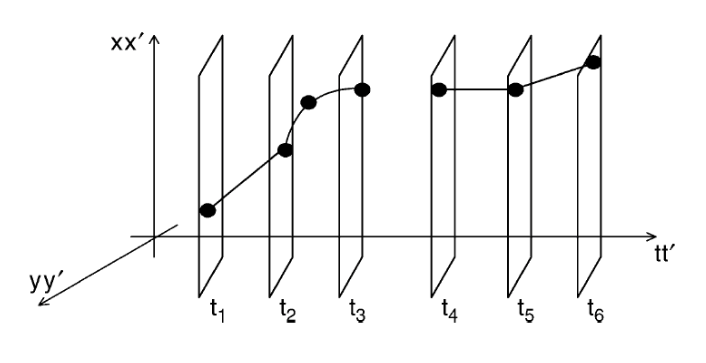
\includegraphics[width=10cm]{sliced}
  \caption{\footnotesize{\emph{Sliced representation} di un oggetto in movimento.}}
  \label{fig:sliced}
\end{figure}
Come presentato in \cite[capitolo~3.1]{mdme}, una definizione teorica del movimento di un oggetto può essere quella di una funzione dallo spazio temporale $I\subseteq\mathbb{R}$ allo spazio geografico $S\subseteq\mathbb{R}^2$:
$$I\subseteq\mathbb{R} \rightarrow S\subseteq\mathbb{R}^2 : t \rightarrow l(t)$$
dove con $l(t)$ si intende la posizione in cui si trova l'oggetto all'istante $t$. in questo modo la traiettoria effettiva seguita da un oggetto può essere definita come:
$$T_{act} = \{t, l(t) | t\in\mathbb{I}\} \subset \mathbb{R}^2\times\mathbb{R}$$
Questo rappresenta una curva continua nella reltà, tuttavia la forma che ci si trova a raprresentare nei calcolatori è la sua versione finita, definita come sequenza di coppie di valori spazio-tempo:
$$T = \{<p_1, t_1>, <p_2, t_2>, ... , <p_n, t_n>\}$$
dove $p_i\in\mathbb{R}^2, t_i\in\mathbb{R}, 1 <= i <= n$ e $t_1 < t_2 < ... < t_n$.
Il risultato è che una traiettoria può essere rappresentata con un modello che si definisce \emph{sliced representation} come quello in figura \ref{fig:sliced}.
Questo modello decompone lo sviluppo temporale in frammenti definiti \emph{slice}, tali per cui questa evoluzione può essere descritta da una qualche funzione semplice, ad esempio l'interpolazione lineare.

\begin{figure}[h]
  \centering
  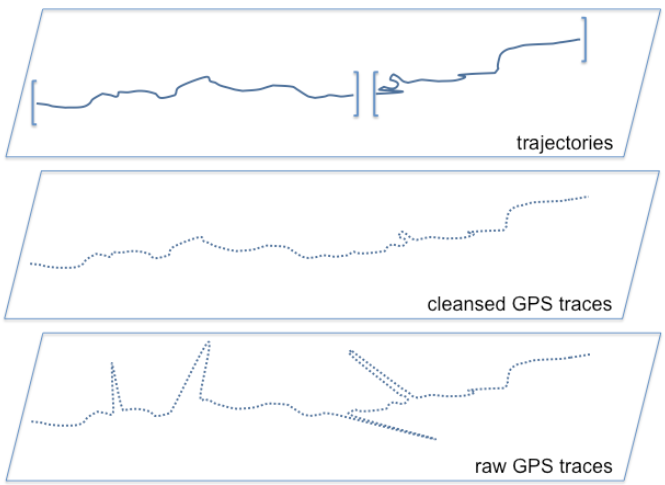
\includegraphics[width=10cm]{rawgps}
  \caption{\footnotesize{Il processo di \emph{trajectory reconstruction} da dati grezzi GPS.}}
  \label{fig:rawgps}
\end{figure}

In generale il problema di \emph{trajectory recontruction} si decompone di due operazioni principali:
\begin{itemize}
\item \emph{data cleansing}: è la fase in cui si ripuliscono i dati grezzi dai segnali di rumore o dagli eventuali \emph{outlier}, è possibile eseguire operazioni di arrotondamento o altre elaborazioni;
\item \emph{trajectory identification}: ha l'obiettivo di interpolare la sequenza di posizioni raccolte al fine di approssimare il movimento continuo dell'oggetto.
\end{itemize}
In particolare per la seconda operazione le modalità sono tutt'altro che semplici e delineate. Sono disponibili diversi approcci, alcuni che si basano sulle caratteristiche geometriche della rappesentazione dei dati, altri si basano su sistemi probabilistici, altri ancora sono sistemi ibridi.

Anche in \emph{PathS} si incontra la problematica fondamentale di ricostruire le traiettorie individuate dai campionamenti. L'approccio che si è valutato più opportuno (considerate le caratteristiche dei dati sorgente) è stato quello di utilizzare un algoritmo di \emph{map matching}.
Il caso di \emph{trajectory reconstruction} che si affrontato è stato quindi quello di ricondurre ciascun campionamento ad una posizione corrispondente nella rete di trasporto. Utilizzando la rappresentazione di grafo $G=(V,E)$ composto di archi e vertici, per ciascuna posizione $<p_i, t_i>$ della traiettoria che non appartiene alla rete, si è individuata la corrispondente coppia $<p_i^i, t_i^i>$ in cui $p_i^i \in e_j$.

\section{Versione precedente e lavori correlati}
L'idea di sviluppo del progetto non è del tutto nuova, ma prende spunto da un lavoro precedente svolto sempre all'interno dell'Università di Padova dallo studente Lorenzo Teodori seguito dal Prof. Palazzi. Il progetto chiamato \emph{Path2.0} voleva essere un sistema partecipativo per fornire indicazioni di navigazione accessibile per utenti con disabilità. L'idea di base è quella sviluppata in \emph{PathS}, ovvero raccogliere informazioni da un insieme di utenti per poi riutilizzarle nel suggerire dei percorsi pedonali. Gli obiettivi in cui questo progetto estende e sviluppa l'idea iniziale sono i seguenti:
\begin{itemize}
\item estendere il concetto di informazione aggiuntiva sul percorso, non trattare solo l'accessibilità (valori $1$, $0$) ma delle \emph{label} più generiche;
\item implementare soluzioni che rispondessero con percorsi diversi dal semplice percorso accessibile e percorso breve;
\item fornire una base di dati elaborati che consenta non solo il \emph{routing}, ma anche l'analisi o l'applicazione ad altri scenari in chiave sociale.
\end{itemize}
Dal punto di vista tecnologico, si è preferito fare tesoro del'esperienza precedente e strutturare un sistema completamente nuovo per le seguenti motivazioni:
\begin{itemize}
\item il sistema SDK utilizzato nello sviluppo dell'applicazione \emph{mobile} era molto datato, richiedeva un profondo aggiornamento e la revisione di alcune modalità di sviluppo;
\item tutta la soluzione era molto legata e del tutto dipendente dai sevizi API di Google Maps (anch'essi da aggiornare);
\item il progetto di partenza non presentava dei caratteri architetturali sufficientemente delineati da consentirne l'utilizzo come base, in particolare per le esigenze di espansione ed evoluzione ad altri contesti;
\end{itemize}

Un progetto analogo a \emph{PathS} nel quale si utilizza però il microfono del dispositivo è Crowd++ \cite{crowdplusplus}. Lo scopo dell'applicazione sviluppata è di individuare dati aggiuntive riguardo l'attività sociale dell'utente e l'interazione tra \emph{speaker} e pubblico in un evento. I suoni registrati dal microfono sono utilizzati per individuare il numero di parole pronunciate o il numero di persone che stanno parlando, cercando quindi di derivare le informazioni necessarie.
Altro esempio da cui si è tratto spunto è il progetto PartecipAct \cite{participact}. Sviluppato recentemente presso l'Università di Bologna, anch'esso ha come obiettivo quello di studiare il potenziale inesplorato della collaborazione tra utenti, sfruttando gli smartphone come strumento di interazione e interconnessione. Coinvolgendo studenti e volontari in un esperimento di raccolta dati, si sono raccolte informazioni sugli utenti e sul contesto in cui si trovano. Tutti i dati vengono memorizzati in un database online cercando rispondere a domande del tipo: ``dove passano la maggior parte del tempo i nostri utenti?''. Come vediamo l'approccio è molto simile a quello di \emph{PathS}, nonostante le modalità di svolgimento e il fine ultimo siano diversi.
